\section{Hierarchical Task Networks}
\label{sec:HTNPlanning}
Classical planning has many shortcomings; for example, 
it views plans as a linear sequence of actions, but it was clear from the early stages of research\cite{NonlinearNaturePlanssacerdoti1975} that planners can solve some problems much better when plans are not constrained by the limitations of linearity. If a planner is capable of reasoning about nonlinear plans, it can delay committing to a specific order of actions until sufficient information is gathered. This can alleviate the need for an exhaustive search of all possible plan orderings. Another big problem with classical planners is the fact that they are easily overwhelmed by complex domains \cite{PracticalPlanningExtendingwilkins1989}. The lack of abstraction levels makes it hard to consider meta-level reasoning. While it is feasible to integrate expert knowledge into the search algorithms, it is not easy, and steering the trajectory of execution is also not a simple task.

Hierarchical task network (HTN) planning tries to overcome some of those shortcomings by introducing more abstraction layers and using expert knowledge to guide the planning process. HTN is based on the premise that goal states as objectives are usually unnatural, and composing abstract actions from smaller concrete sub-actions is much more intuitive. Furthermore, having the domain knowledge organized hierarchically will allow the planner to create plans using action reduction, meaning the most important conditions will be considered first, and the details will be considered later in the planning process \cite{FormalizingPlanningKnowledgeyang1990}.

The abstraction that HTN introduces is implemented using two types of constructs \cite{PANDAFrameworkHierarchicalholler2021}: primitive and compound tasks. These constructs are combined to form partially ordered sets called task networks. The primitive tasks are comparable to actions in classical planning; they can be executed if the current state of the environment adheres to some condition and they have some effect on the environment. The compound tasks represent more complex actions that cannot be executed in one step and must be decomposed using some decomposition method. The decomposition methods are part of the planning domain, and each method can decompose a specific compound task into a task network. Multiple methods can decompose one compound task; in contrast, there is a one-to-one mapping between operators and primitive tasks.


\subsection{Formal Definitions}
Throughout the years, numerous attempts have been made to establish a standard formalism for HTN planning \cite{bercher_survey_2019}. Some of these approaches were actually unique, while others were essentially comparable. The purpose of this section is not to provide a comprehensive formal framework but rather to provide a formal background that will assist the reader in comprehending HTN's underlying structure. The following formal structures are derived from \cite{OverviewHierarchicalTaskgeorgievski2014} \cite{alnazer2019htn}.

\begin{Tdef}[Primitive task]
    A primitive task  $t_p \in T_p$ is a pair $t_p = <symbol(t_p),terms(t_p)>$, where:
    \vspace{-0.5em}
    \begin{compactitem}
    \item 
    $T_p$ is a finite set of primitive tasks.
    \item 
    $symbol(t_p)$ is a primitive task symbol.
    \item 
    $terms(t_p)$  is a set of terms, such that $terms(t_p) = \langle \tau_1, \tau_2, \dots, \tau_n \rangle$.
    \end{compactitem}
\end{Tdef}

\begin{Tdef}[Operator]
    An operator $o \in O$ is a triple $o = <p(o), pre(o), eff(o)>$, where:
    \vspace{-0.5em}
    \begin{compactitem}
    \item 
    $O$ is a finite set of operators.
    \item 
    $p(o)$ is a primitive task.
    \item 
    $pre(o)$ and $eff(o)$ are precondition and effect.
    \end{compactitem}
    It is important to remember that each primitive task must have one and only one operator, but multiple primitive tasks can utilize a single operator. An operator is quite comparable to an action from classical planning. We say an operator $o$ is applicable in a state $s$ if and only if:
    \vspace{-0.5em}
    $$\forall p_i \in pre(o): p_i\in s \text{ and } \forall \bar{p_i} \notin s$$
\end{Tdef}

\begin{Tdef}[Compound task]
    A compound task $t_c \in T_c$ is a pair $t_c = <symbol(t_c),terms(t_c)>$, where:
    \vspace{-0.5em}
    \begin{compactitem}
    \item 
    $T_c$ is a finite set of compound tasks.
    \item 
    $symbol(t_c)$ is a compound task symbol.
    \item 
    $terms(t_c)$  is a set of terms, such that $terms(t_c) = \langle \tau_1, \tau_2, \dots, \tau_n \rangle$.
    \end{compactitem}

    In practice, it is often beneficial to extend this definition to include a set of preconditions $pre(t_c)$ that must hold in the current world state for the planner to even consider this compound task for decomposition.
\end{Tdef}

\begin{Tdef}[Task network]
    A task network $tn$ is a pair $<T, \prec>$ , where:
    \vspace{-0.5em}
    \begin{compactitem}
    \item 
    $T$ is a finite set of tasks.
    \item 
    $\prec$ is a partial order on $T$.
    \end{compactitem}
\end{Tdef}

\begin{Tdef}[Method]
    A method $m \in M$ is a triple $m = <c(m), pre(m), tn(m)>$, where:
    \vspace{-0.5em}
    \begin{compactitem}
    \item 
    $M$ is a set of methods.
    \item 
    $c(m)$ is a compound task.
    \item 
    $pre(m)$ is a precondition.
    \item 
    $tn(m)$ is a task network.
    \end{compactitem}
    A method $m$ is applicable in a state $s$ if and only if:
    \vspace{-0.5em}
    $$\forall p_i \in pre(m): p_i\in s \text{ and } \forall \bar{p_i} \notin s$$
\end{Tdef}

\begin{Tdef}[Decomposition]
   Given a task network $tn=<T, \prec>$, and an applicable method $m$ for a compound task $t= c(m)$, we say that $m$ decomposes $tn$ into $\acute{tn}$ with:
   \vspace{-0.5em}
    \begin{compactitem}
    \item 
    $\acute{tn} = ((T \setminus\{ t \}) \cup T_m, \prec \cup \prec_m \cup \prec_D) $ where 
    \item 
    $\prec_D = \{ (t_1, t_2) \in T \times T_m | (t_1, t) \in  \prec\} \cup \{ (t_1, t_2) \in T_m \times T | (t, t_2) \in  \prec\}$ 
    \end{compactitem}
\end{Tdef}


\begin{Tdef}[HTN planning domain]
    A  HTN planning domain is a pair $\Sigma= (O, M)$ where:
    \vspace{-0.5em}
    \begin{compactitem}
    \item 
    $O$ is a set of operators.
    \item 
    $M$ is a set of methods.
    \end{compactitem}
\end{Tdef}

\begin{Tdef}[HTN planning problem]
    A HTN planning problem is a triple $\pi = (\Sigma,s_0,tn_0)$, where:
    \vspace{-0.5em}
    \begin{compactitem}
    \item 
    $\Sigma$ is the planning domain.
    \item 
    $s_0$ is the initial state.
    \item 
    $tn_0$ is the initial task network.
    \end{compactitem}
\end{Tdef}

\subsubsection{Planners}
There are numerous strategies implemented by different HTN planners to solve an HTN planning problem. HTN planners can be classified based on the search space in which the planner operates. This work is not intended to provide a full overview of HTN planners, as has been done in \cite{bercher_survey_2019} and \cite{OverviewHierarchicalTaskgeorgievski2014}. Therefore, we will only provide an oversimplified overview of how HTN planners function. HTN planners are fundamentally different from classical planners in that they do not pursue some goal state but rather try to simplify a hierarchical network of tasks into a linear sequence of \qq{actions}. Some HTN planners perform a decomposition-based search, in which applicable methods repeatedly decompose the task network until no more compound tasks are left. The result would be a task network that consists of only primitive tasks. Others perform a progression-based search, where the planner decomposes compound tasks and executes primitive tasks when applicable until the task network is empty. It is important to know that decomposing a compound task changes the structure of the task network but not the state. On the other hand, executing a primitive task changes the state of the environment but not the structure of the task network. When performing a progression-based search, the planner must keep track of the executed primitive tasks; otherwise, it is necessary to retrace the path the planner took from the initial task network to the empty one.

\subsubsection{Description Languages}
Using a description language, HTN planning domains and problems can be described just as they are in classical planning. Prolog\footnote{\url{https://en.wikipedia.org/wiki/Prolog}} is commonly used, especially in academic research. PDDL has also been extended to support HTN constructs. Recently a new description language based on PDDL called HDDL (Hierarchical Domain Definition Language) has been adopted as the standard input language for the track on hierarchical planning at the International Planning Competition. Planners are typically reluctant to adopt new formats; currently, most planners only support a custom input format. HPDL and TF are two older formats that might be encountered. However, they are no longer widely utilized.

%\begin{figure}[h]
%    \centering
%    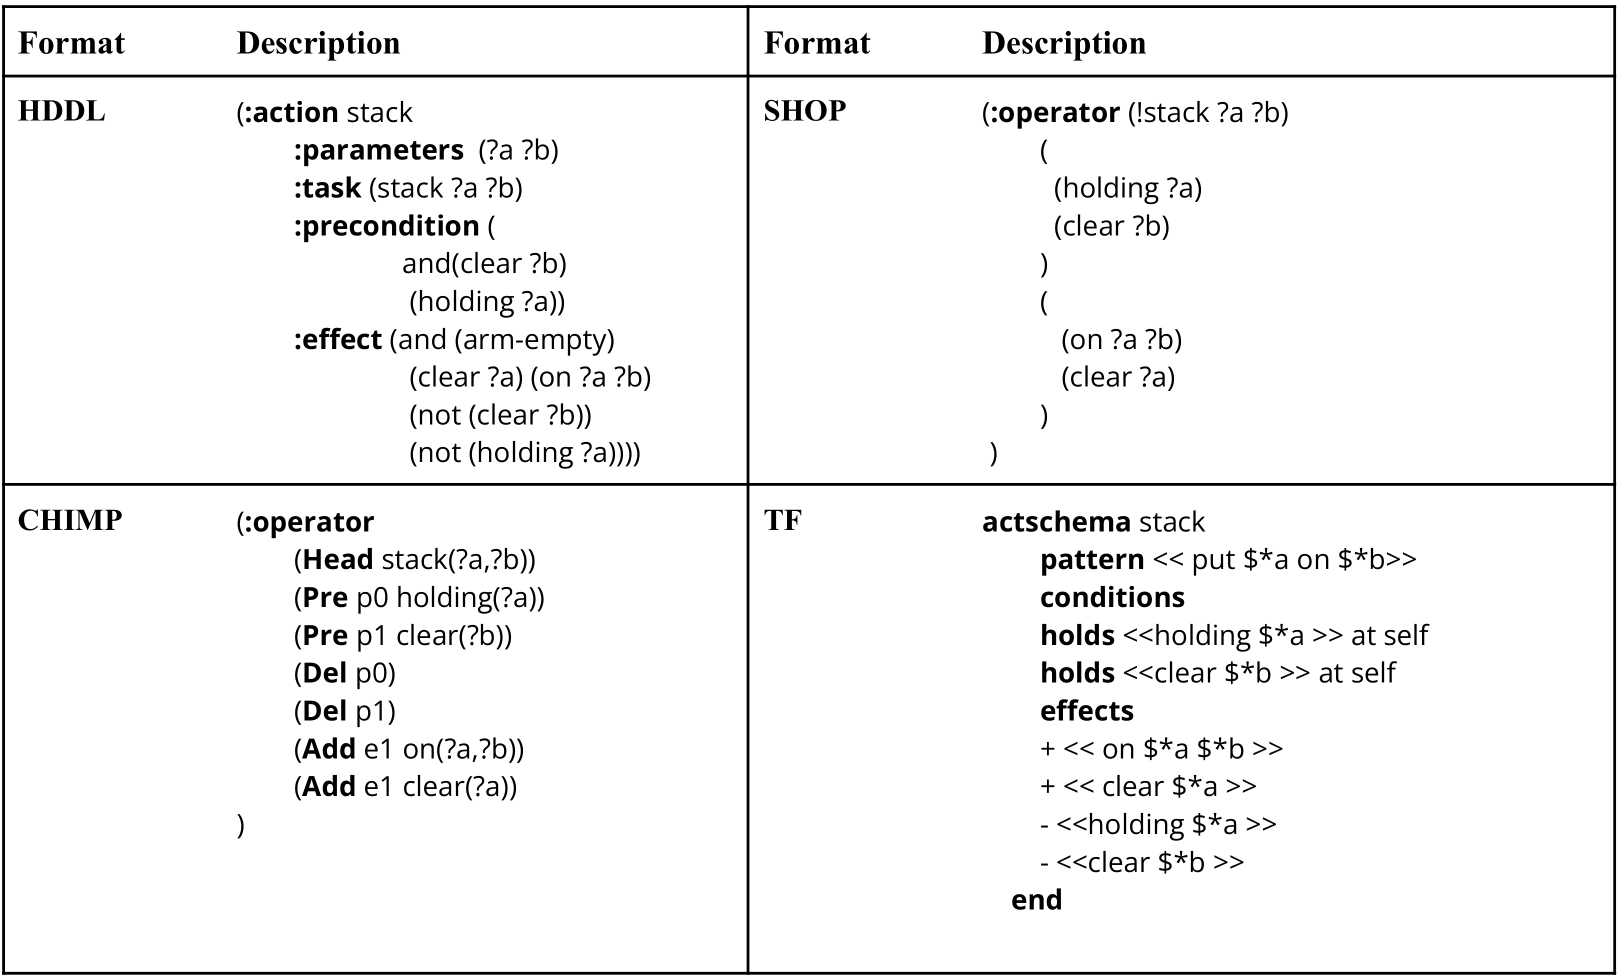
\includegraphics[width=\textwidth]{graphics/formats.png}
%    \caption{The stack task from the block-world domain in different formats.}
%    \label{fig:formats}
%\end{figure}

\begin{table}[H]
    \centering
    \resizebox{\textwidth}{!}{%
    \begin{tabular}{|m{0.1\textwidth}m{0.4\textwidth}|m{0.1\textwidth}m{0.4\textwidth}|}
    \hline
    \textbf{Planner} & \textbf{Description} & \textbf{Planner} & \textbf{Description} \\\hline
    \textbf{HDDL} & \begin{lstlisting}[
    basicstyle={\small\ttfamily},
  numbers=left,
  numberstyle=\tiny\color{gray},
  breaklines=true,
  breakatwhitespace=true,
  tabsize=3,
  language=HDDL
]
(:action stack
  :parameters  (?a ?b)
  :task (stack ?a ?b)
  :precondition (
                  and(clear ?b)
                  (holding ?a))
  :effect (and (arm-empty)
               (clear ?a) (on ?a ?b)
               (not (clear ?b))
               (not (holding ?a))))
\end{lstlisting} & \textbf{SHOP} & \begin{lstlisting}[
    basicstyle={\small\ttfamily},
  numbers=left,
  numberstyle=\tiny\color{gray},
  breaklines=true,
  breakatwhitespace=true,
  tabsize=3,
  language=JSHOP,
]
(:operator (!stack ?a ?b)
  (
    (holding ?a)
    (clear ?b)
  )
  (
    (on ?a ?b)
    (clear ?a)
  )
)
\end{lstlisting} \\ \hline
    \textbf{CHIMP} & \begin{lstlisting}[
    basicstyle={\small\ttfamily},
  numbers=left,
  numberstyle=\tiny\color{gray},
  breaklines=true,
  breakatwhitespace=true,
  tabsize=3,
  language=CHIMP
]
(:operator
        (Head stack(?a,?b))
        (Pre p0 holding(?a))
        (Pre p1 clear(?b)) 
        (Del p0)
        (Del p1)
        (Add e1 on(?a,?b))
        (Add e1 clear(?a))
)
\end{lstlisting} & \textbf{TF} & \begin{lstlisting}[
    basicstyle={\small\ttfamily},
  numbers=left,
  numberstyle=\tiny\color{gray},
  breaklines=true,
  breakatwhitespace=true,
  tabsize=3,
  language=TF
]
actschema stack
  pattern << put $*a on $*b>>
  conditions
  holds <<holding $*a >> at self
  holds <<clear $*b >> at self
  effects
  + << on $*a $*b >>
  + << clear $*a >>
  - <<holding $*a >>
  - <<clear $*b >>
end
\end{lstlisting} \\ \hline
    \end{tabular}%
    }
    \caption{The stack task from the block-world domain in different formats.}
    \label{tab:my-table}
\end{table}



There are also planners that use a programming language to describe the domain and problem rather than a specialized description language. This approach has the advantage that the planner can be directly integrated into the system without needing a translation layer between the system and the planner. RAE\footnote{\url{https://github.com/patras91/rae_release}}, GTPyhop\footnote{\url{https://github.com/dananau/GTPyhop}} and FluidHTN\footnote{\url{https://github.com/ptrefall/fluid-hierarchical-task-network}} are all great examples of this approach.

\begin{Listing}
    \begin{lstlisting}[language=Python]
        def stack(s,b1,b2):
            if s.pos[b1] == 'hand' and s.clear[b2] == True:
                s.pos[b1] = b2
                s.clear[b1] = True
                s.holding['hand'] = False
                s.clear[b2] = False
                return s
    \end{lstlisting}
    \caption{The stack task from the block-world domain in GTPyhop.}
    \label{lst:StackPython}
\end{Listing}